\documentclass{article}

\usepackage[T1]{fontenc}
\usepackage[utf8]{inputenc}
\usepackage[brazilian]{babel}
\usepackage{graphicx}
\usepackage[export]{adjustbox}[2011/08/13]
\usepackage{float}
\usepackage[pdftex]{hyperref}
\usepackage{epstopdf}
\usepackage{etoolbox}
\usepackage{amsmath}
\usepackage{amsfonts}
\usepackage{amssymb}
\usepackage{caption}
\usepackage{subcaption}
\usepackage{setspace}
\usepackage{tikz}
\usepackage{listings}
\usepackage{xcolor} 
\usepackage{multirow}

\bibliographystyle{eric}
\patchcmd{\thebibliography}{\section*}{\section}{}{}


\newcommand{\R}{\ensuremath{\mathbb{R}}}
\newcommand{\Prob}{\ensuremath{\mathbb{P}}}
\newcommand{\K}{\ensuremath{\mathbb{K}}}
\newcommand{\U}{\ensuremath{\mathbb{U}}}
\newcommand{\N}{\ensuremath{\mathbb{N}}}
\newcommand{\Lg}{\ensuremath{\mathbb{L}}}
\newcommand{\T}{\ensuremath{\rm Tr}}
\newcommand{\sg}{{\sigma(x_k)}}

\newcommand{\G}{\ensuremath{\mathcal{G}}}
\newcommand{\F}{\ensuremath{\mathcal{F}}}
\newcommand{\C}{\ensuremath{\mathcal{C}}}
\newcommand{\E}{\ensuremath{\mathcal{E}}}
\newcommand{\Hn}{\ensuremath{\mathcal{H}}}
\newcommand{\Hoo}{\ensuremath{\mathcal{H}_\infty}}
\newcommand{\Hop}{\ensuremath{\mathcal{H}_{op}}}
% --------------------------------------------------
\newtheorem{theo}{Teorema}
\newtheorem{exa}{Exemplo}
\newtheorem{lemm}{Lema}
\newtheorem{coro}{Corolário}
\newtheorem{defn}{Definição}[section]


\DeclareCaptionType{capequ}[Equação][]
\captionsetup[capequ]{labelformat=empty}

\begin{document}

\begin{titlepage}
\begin{center}

\newcommand{\HRule}{\rule{\linewidth}{0.5mm}}
% Upper part of the page. The '~' is needed because \\
% only works if a paragraph has started.

\includegraphics[width=0.15\textwidth]{logoUnicamp}~\\[1cm]

\textsc{\LARGE Universidade Estadual de Campinas}\\[1.5cm]

\textsc{\Large Faculdade de Engenharia Mecânica}\\[0.5cm]

% Title
\HRule \\[0.4cm]
{ \huge \bfseries ES664 - Laboratório de Eletrônica para Automação Industrial\\ \vspace{1cm} Relatório - Experimento 4\\
\Large{Acionamento de motor DC} \\[0.4cm] }

\HRule \\[1.5cm]

% Author and supervisor
\begin{minipage}{0.6\textwidth}
\begin{flushleft} \large
\emph{Nome:}\\
Daniel Dello Russo Oliveira\\Marcelli Tiemi Kian
\end{flushleft}
\end{minipage}
\begin{minipage}{0.2\textwidth}
\begin{flushright} \large
\emph{RA}\\ 101918\\117892
\end{flushright}
\end{minipage}

\vfill

% Bottom of the page
{\large \today}

\end{center}
\end{titlepage}


\onehalfspacing
\section{Objetivos}
	Esse experimento tem como objetivo o estudo de um conversor DC-DC de topologia reversível (buck/boost) e o efeito do duty-cycle na sua tensão de saída.

\section{Conversor Buck}
Conectamos o kit didático para trabalhar e modo step-down conforme detalhado na figura \ref{fig:buesq}.
\begin{figure}[H]
	\centering
	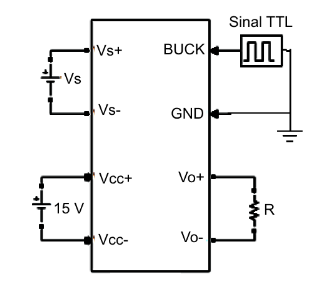
\includegraphics[width=0.5\linewidth]{Dados/buck/esq}
	\caption{Conexões do chopper reversível em modo step-down \cite{bb:paiva}}
	\label{fig:buesq}
\end{figure}
Com $V_s = 12V$ e o sinal $TTL$ um trem de pulsos de $0$ a $5V$ DC com frequência de $3kHz$ e duty-cycle de $50\%$.

Medimos então a curva de corrente no indutor através do sensor ACS756 que pode ser visualizada na figura \ref{fig:buil}
\begin{figure}[H]
	\centering
	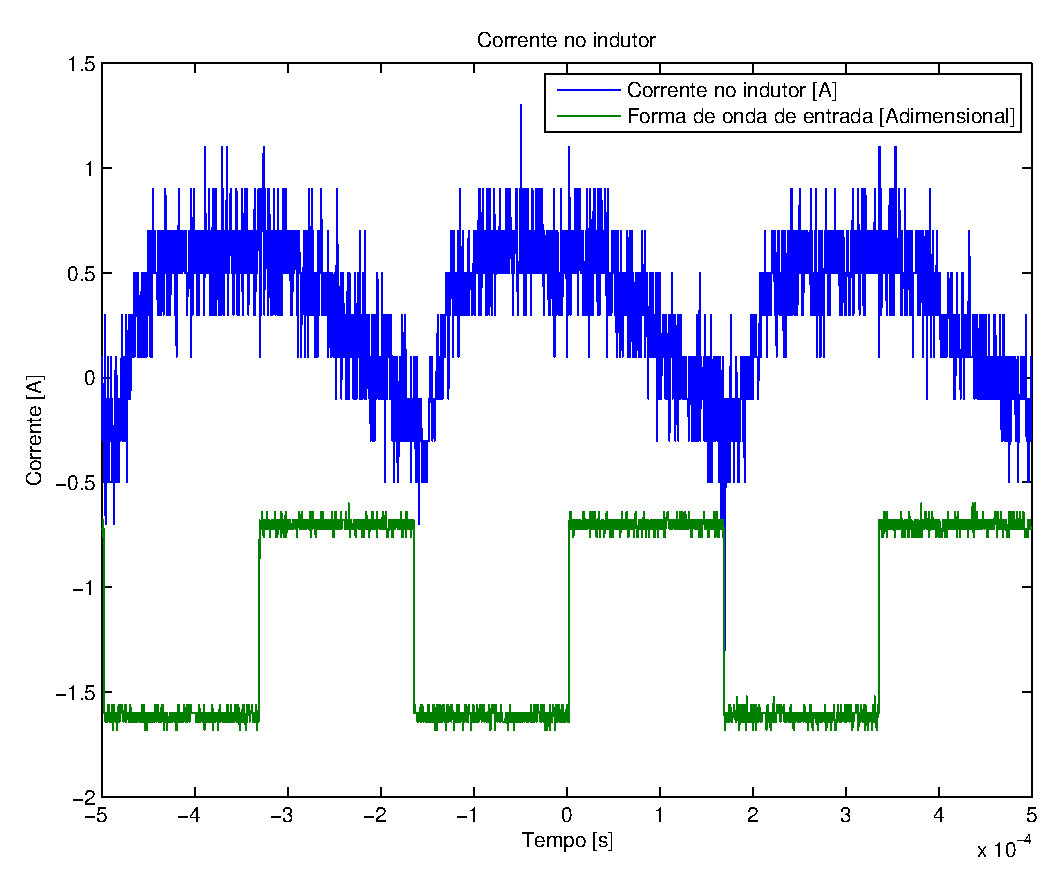
\includegraphics[width=0.5\linewidth]{Dados/buck/il}
	\caption{Curvas de corrente no indutor para conversor buck}
	\label{fig:buil}
\end{figure}
Como podemos ver estamos operando em modo de condução descontínua (a corrente no indutor chega a 0). O valor médio assumido pela corrente no indutor foi de aproximadamente $0.25 A$

Medimos também a tensão de saída do conversor, apresentada na figura \ref{fig:but3k}
\begin{figure}[H]
	\centering
	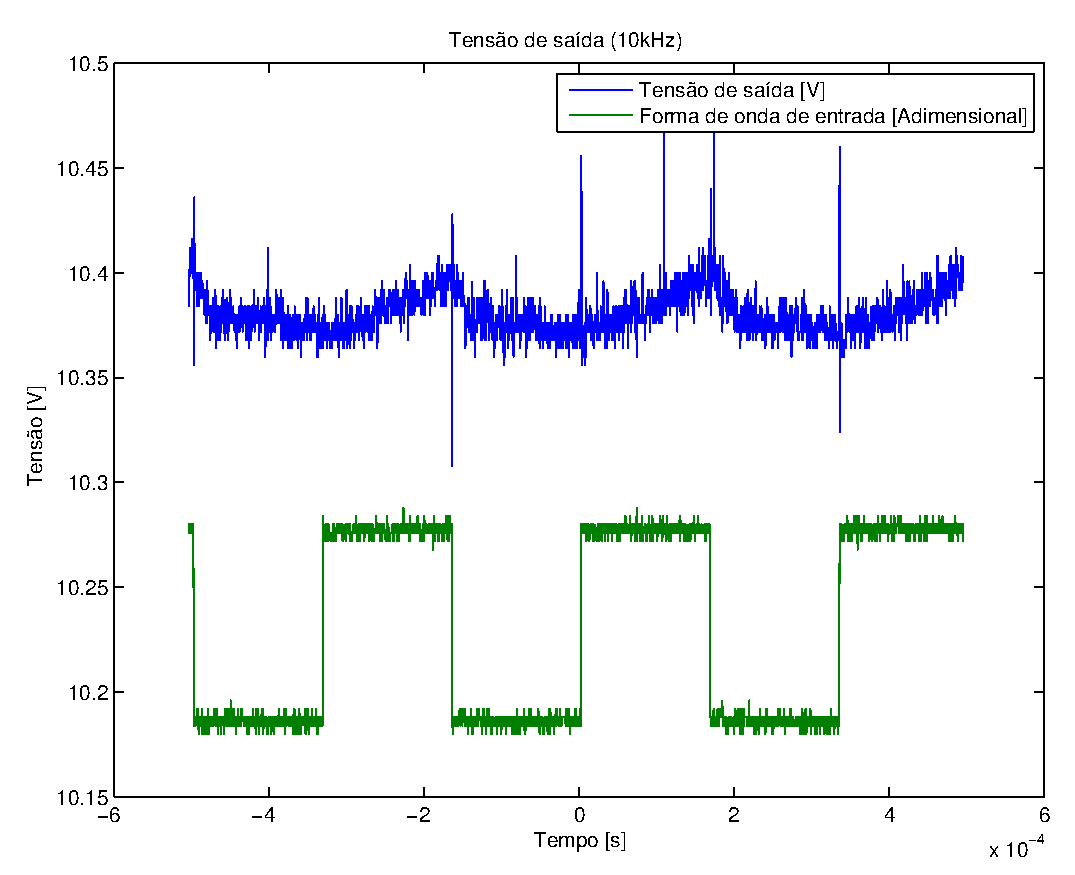
\includegraphics[width=0.5\linewidth]{Dados/buck/t3k}
	\caption{Tensão de saída conversor buck (3 kHz)}
	\label{fig:but3k}
\end{figure}

O valor médio da tensão de saída foi de $10.3 V$. Armados desses dados, do conhecimento de que o conversor estava trabalhando em modo de condução descontínua e da equação \ref{eq:bud} encontramos o valor da indutância de nosso kit didático: $L \approx 330.1 \mu H$

\begin{capequ}[H]
	\begin{equation}
	\overline{V_R} = V_s\frac{D^2}{D^2 + 2\frac{LI_lf_s}{V_s}}
	\end{equation}
	\caption{Equação da tensão de saída para conversor buck em modo de condução descontínua}
	\label{eq:bud}
\end{capequ}

Variamos o duty-cycle do sinal de controle entre $10$ e $70\%$ e medimos a tensão média sobre a carga. Encontramos uma curva que se aproxima desse sinal e que possui a mesma forma da equação \ref{eq:bud} (equação \ref{eq:bulin}) e calculamos os valores teóricos que essa tensão deveria assumir (supondo modo de condução descontínua e que a corrente média no indutor se manteve aproximadamente $0.25 A$). Os resultados podem ser visualizados na figura \ref{fig:butvd}.

\begin{capequ}[H]
	\begin{equation}
	V_R = 11.36\frac{D^2}{D^2 +  0.02055}	
	\end{equation}
	\caption{Curva que aproxima a tensão medida de saída em função do duty-cycle}
	\label{eq:bulin}
\end{capequ}

\begin{figure}[H]
	\centering
	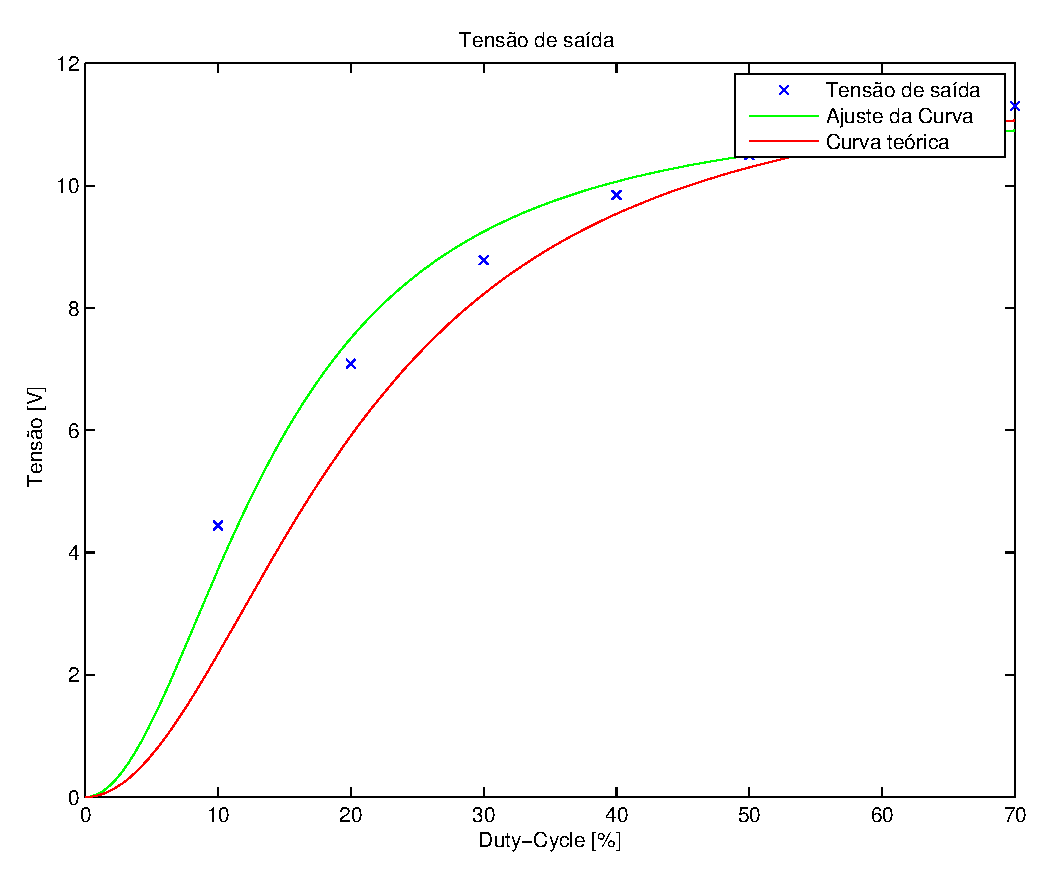
\includegraphics[width=0.7\linewidth]{Dados/buck/tvd}
	\caption{Tensão de saída conversor buck em função do duty-cycle}
	\label{fig:butvd}
\end{figure}

Como podemos ver os valores medidos estão bastante próximos dos esperados teoricamente porém levemente maiores. Isso acontece porque nos cálculos teóricos deixamos de levar em conta uma série de fatores, entre eles o fato dos componentes do circuíto não serem ideais (perdemos energia em vários pontos que não foram levados em conta), o fato da corrente média no indutor variar (fator que ignoramos para simplificar/possibilitar os cálculos), o fato de que a resposta dos componentes nem sempre é imediata entre outros. Também devemos lembrar que existem imprecisões de medida que afetam os resultados obtidos.


\section{Conversor Boost}

Conectamos o kit didático para trabalhar e modo step-up conforme detalhado na figura \ref{fig:boesq}.
\begin{figure}[H]
	\centering
	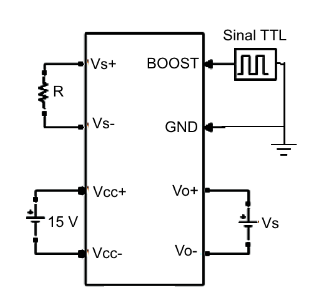
\includegraphics[width=0.5\linewidth]{Dados/boost/esq}
	\caption{Conexões do chopper reversível em modo step-up \cite{bb:paiva}}
	\label{fig:boesq}
\end{figure}
Com $V_s = 5V$ e o sinal $TTL$ um trem de pulsos de $0$ a $5V$ DC com frequência de $3kHz$ e duty-cycle de $50\%$.

Medimos então a curva de corrente no indutor através do sensor ACS756 que pode ser visualizada na figura \ref{fig:boil}
\begin{figure}[H]
	\centering
	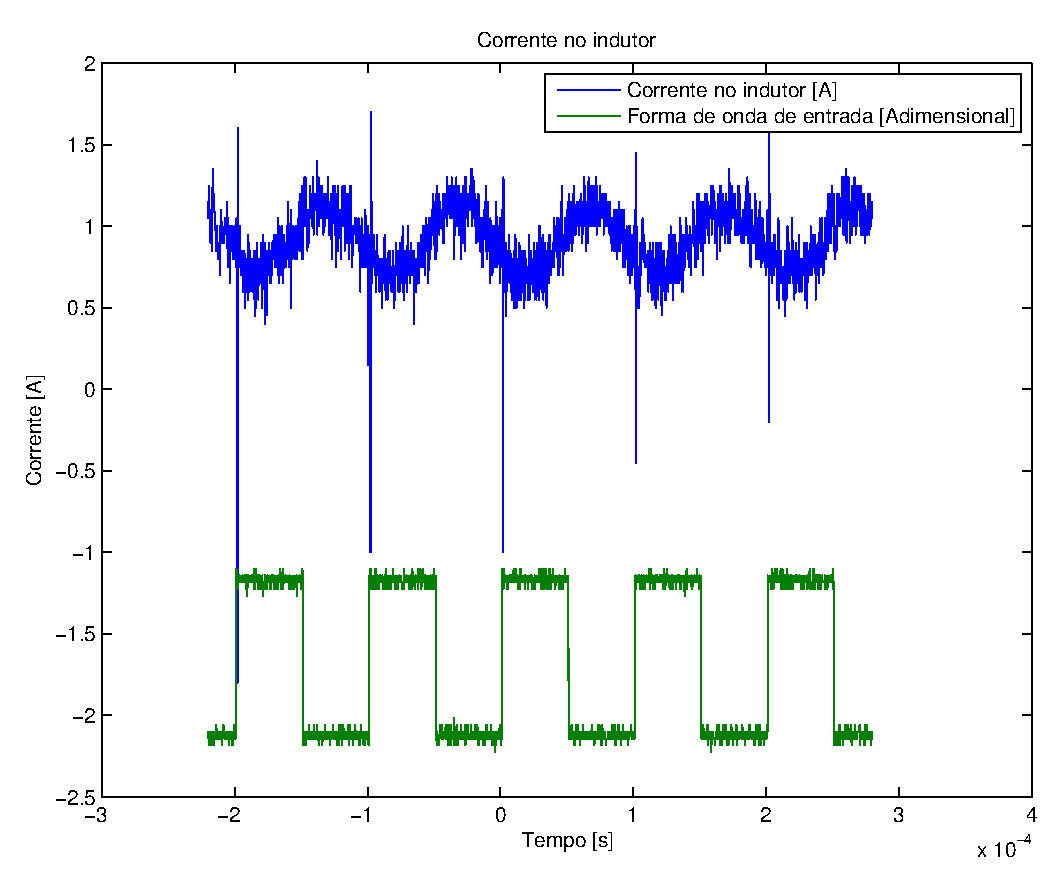
\includegraphics[width=0.5\linewidth]{Dados/boost/il}
	\caption{Curvas de corrente no indutor para conversor boost}
	\label{fig:boil}
\end{figure}
Como podemos ver estamos operando em modo de condução contínua (a corrente no indutor não chega a 0).

Medimos também a tensão de saída do conversor, apresentada na figura \ref{fig:bot3k}
\begin{figure}[H]
	\centering
	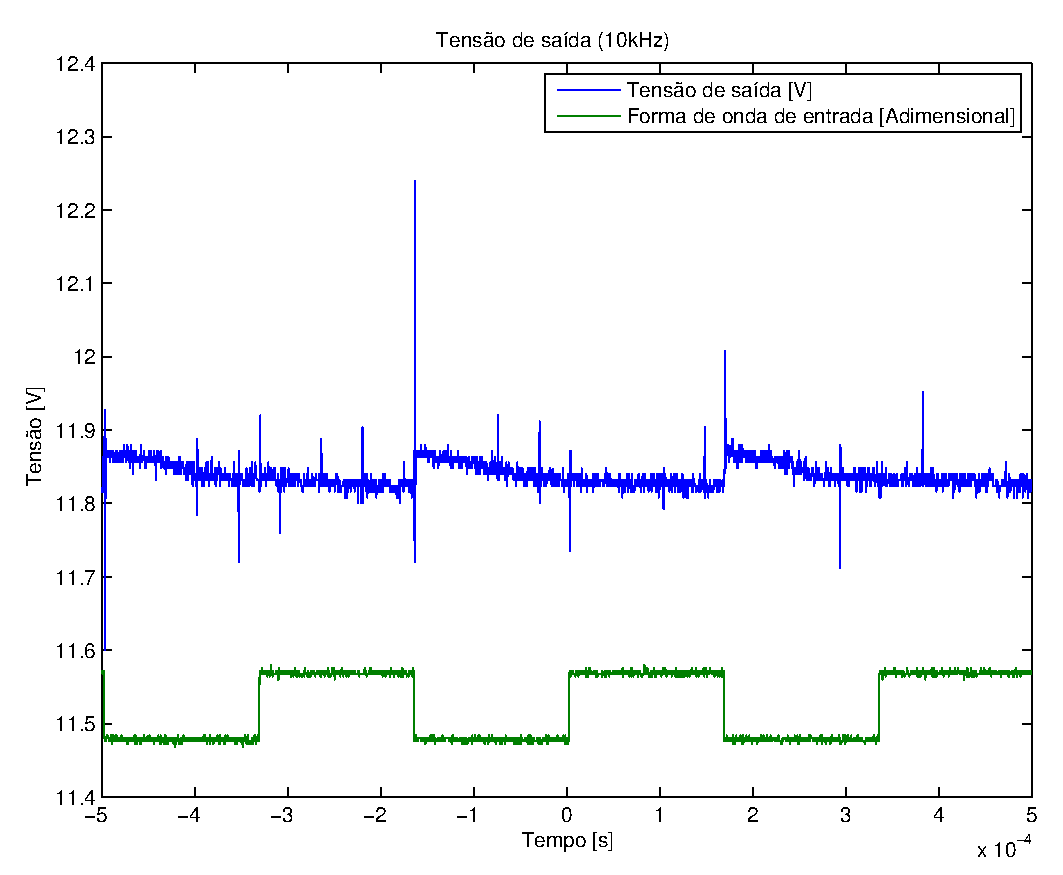
\includegraphics[width=0.5\linewidth]{Dados/boost/t3k}
	\caption{Tensão de saída conversor boost (3 kHz)}
	\label{fig:bot3k}
\end{figure}

O valor médio da tensão de saída foi de $11.9 V$.

Variamos o duty-cycle do sinal de controle entre $20$ e $70\%$ e medimos a tensão média sobre a carga. Encontramos uma curva que se aproxima desse sinal (equação \ref{eq:bolin}) e calculamos os valores teóricos que essa tensão deveria assumir usando a equação \ref{eq:bod} (supondo modo de condução contínua). Os resultados podem ser visualizados na figura \ref{fig:botvd}.

\begin{capequ}[H]
	\begin{equation}
	V_R = \frac{4.623}{1.011 - D}	
	\end{equation}
	\caption{Curva que aproxima a tensão medida de saída em função do duty-cycle}
	\label{eq:bolin}
\end{capequ}

\begin{capequ}[H]
	\begin{equation}
	\overline{V_R} = V_s\frac{1}{1 - D}
	\end{equation}
	\caption{Equação da tensão de saída para conversor boost em modo de condução contínua}
	\label{eq:bod}
\end{capequ}


\begin{figure}[H]
	\centering
	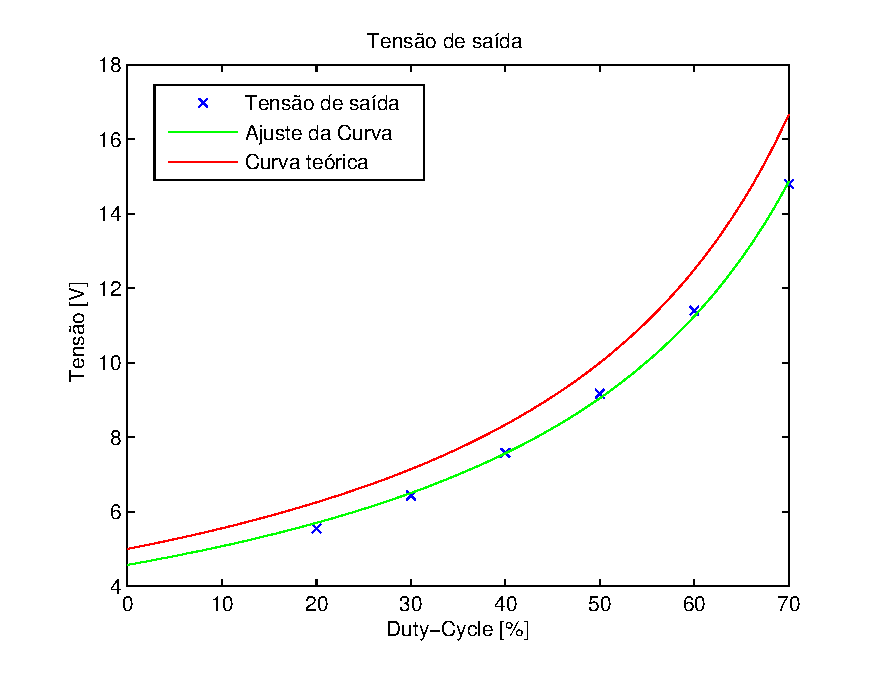
\includegraphics[width=0.7\linewidth]{Dados/boost/tvd}
	\caption{Tensão de saída conversor boost em função do duty-cycle}
	\label{fig:botvd}
\end{figure}

Como podemos ver os valores medidos estão bastante próximos dos esperados teoricamente porém levemente menores. Isso acontece porque nos cálculos teóricos deixamos de levar em conta uma série de fatores, entre eles o fato dos componentes do circuíto não serem ideais (perdemos energia em vários pontos que não foram levados em conta) e o fato de que a resposta dos componentes nem sempre é imediata. Também devemos lembrar que existem imprecisões de medida que afetam os resultados obtidos.

\section{MOSFET IRFZ44}

O transistor utilizado para os conversores do kit é o IRFZ44. Estes MOSFETs possuem rápido chaveamento e baixa resistência em condução, o que viabiliza sua aplicação com os sinais de alta-frequência do gerador de sinais no gate. Conforme utilização no experimento, notamos que não há uma interferência tão significativa por causa do tempo de resposta mesmo chegando aos $10\ kHz$.

De acordo com informativo técnico do dispositivo semicondutor da empresa Vishay, a tensão de ruptura reversa é de $60\ V$, e a tensão de "threshold" $V_{GS}$ é de no mínimo $2\ V$ e no máximo de $4\ V$. Logo, não temos problemas em utilizar a saída do gerador de sinal de amplitude $5\ V$ como entrada do Gate, nem a tensão da fonte na entrada do buck com amplitude de $15\ V$.

\section{Sensor de corrente ACS756}
% Resposta de uma das perguntas, depois ver onde colocar
Para medir a corrente no indutor, utilizamos o sensor ACS756 da Allegro MicroSystems, cujo funcionamento encontra-se detalhado em \cite{bb:allegro}, disponível na placa didática. Esse sensor funciona através de um pequeno trecho condutivo acoplado a um circuito de efeito Hall. Quando existe corrente passando pelo condutor, o circuito Hall converte o campo magnético gerado em uma tensão de saída. 

Para converter essa tensão em corrente, devemos subtraí-la da metade do valor da tensão de alimentação fornecida ao IC (nominalmente $5\ V$ e supomos que essa é a maneira que o aparelho está montado no kit didático) e dividir ela pela sensibilidade do aparelho (podendo ser 20 ou 40 mV/A dependendo do tipo do IC, supomos que o utilizado tenha sensibilidade de 40 mV/A por falta de mais informações). Esse tipo de sensor é mais eficiente energeticamente e interfere menos no circuito medido do que uma resistência de medição interferiria.


\section{Indutância Limite}

Variamos as frequências de chaveamento conforme podemos observar nas figuras \ref{fig:but} e \ref{fig:bot}. nas menores frequências de chaveamento temos maiores tensões médias de saída ($v_R$), e maiores oscilação na sua amplitude.

\begin{figure}[H]
	\begin{subfigure}[b]{0.3\textwidth}
		\centering
		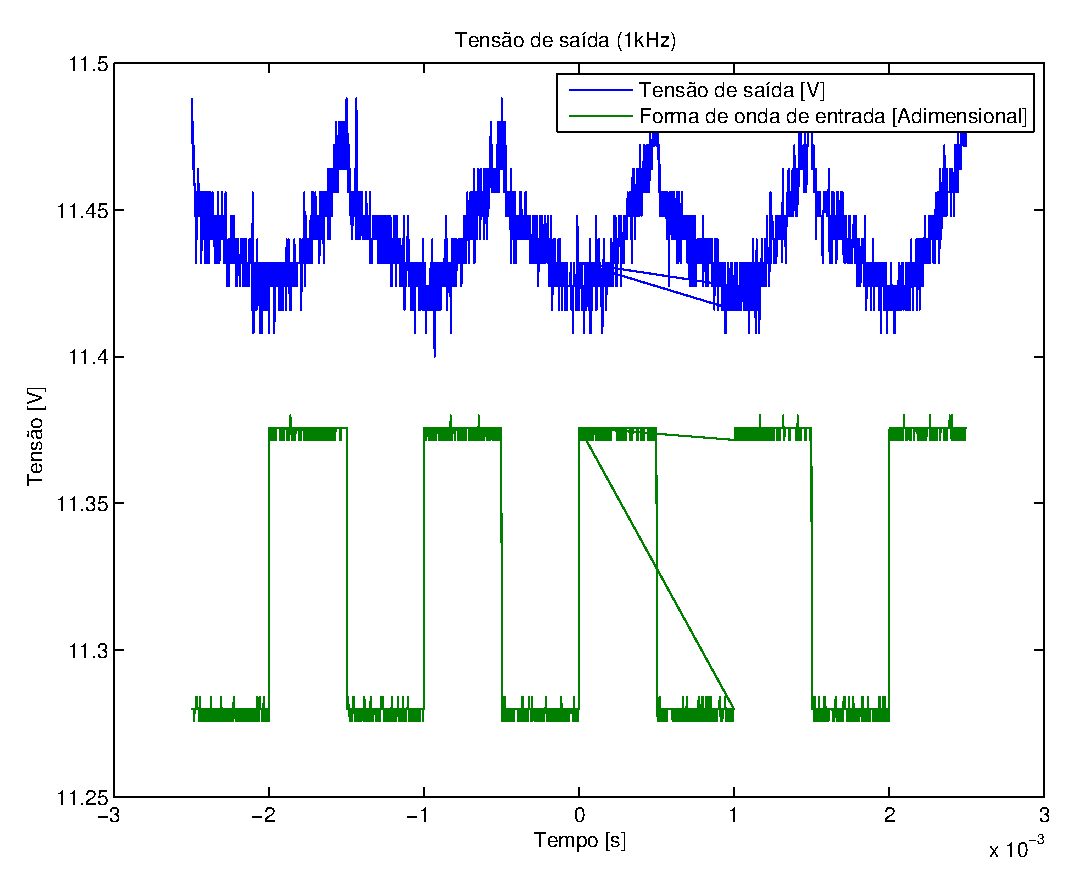
\includegraphics[width=\textwidth]{Dados/buck/t1k}
		\caption{1 kHz}
	\end{subfigure}
	\begin{subfigure}[b]{0.3\textwidth}
		\centering
		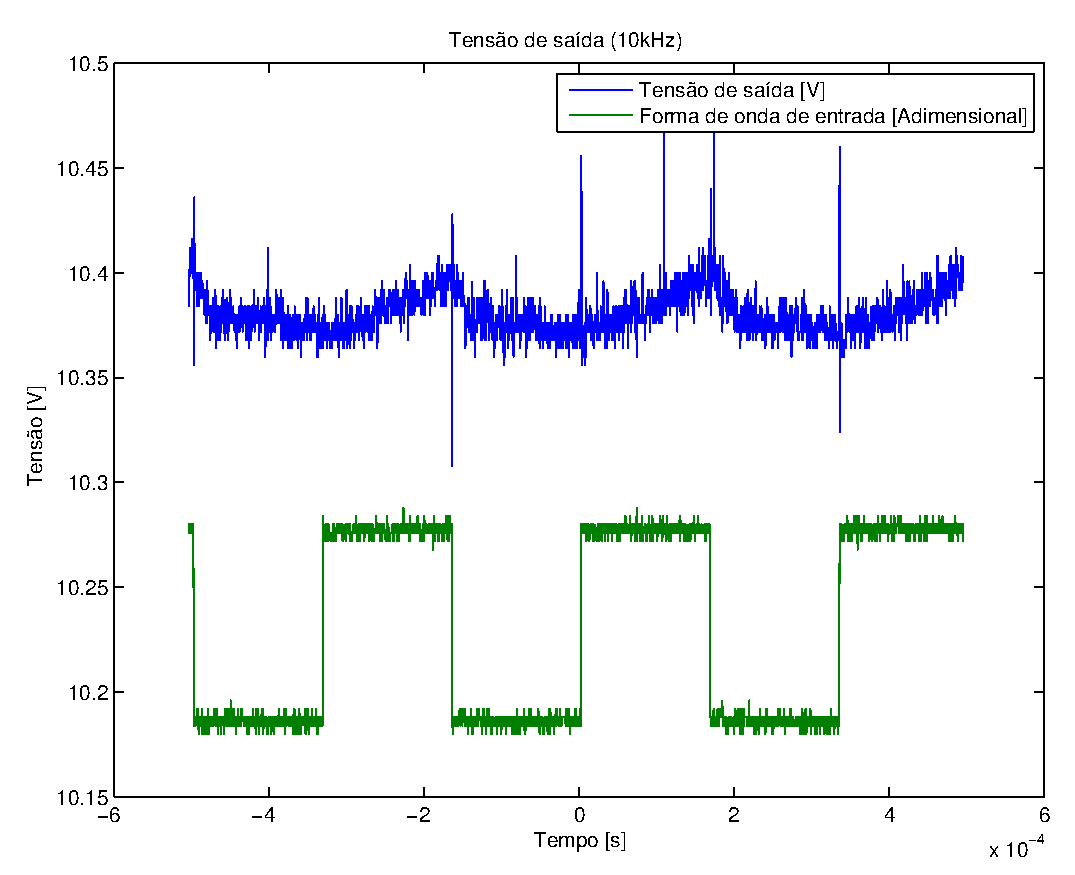
\includegraphics[width=\textwidth]{Dados/buck/t3k}
		\caption{3 kHz}
	\end{subfigure}
	\begin{subfigure}[b]{0.3\textwidth}
		\centering
		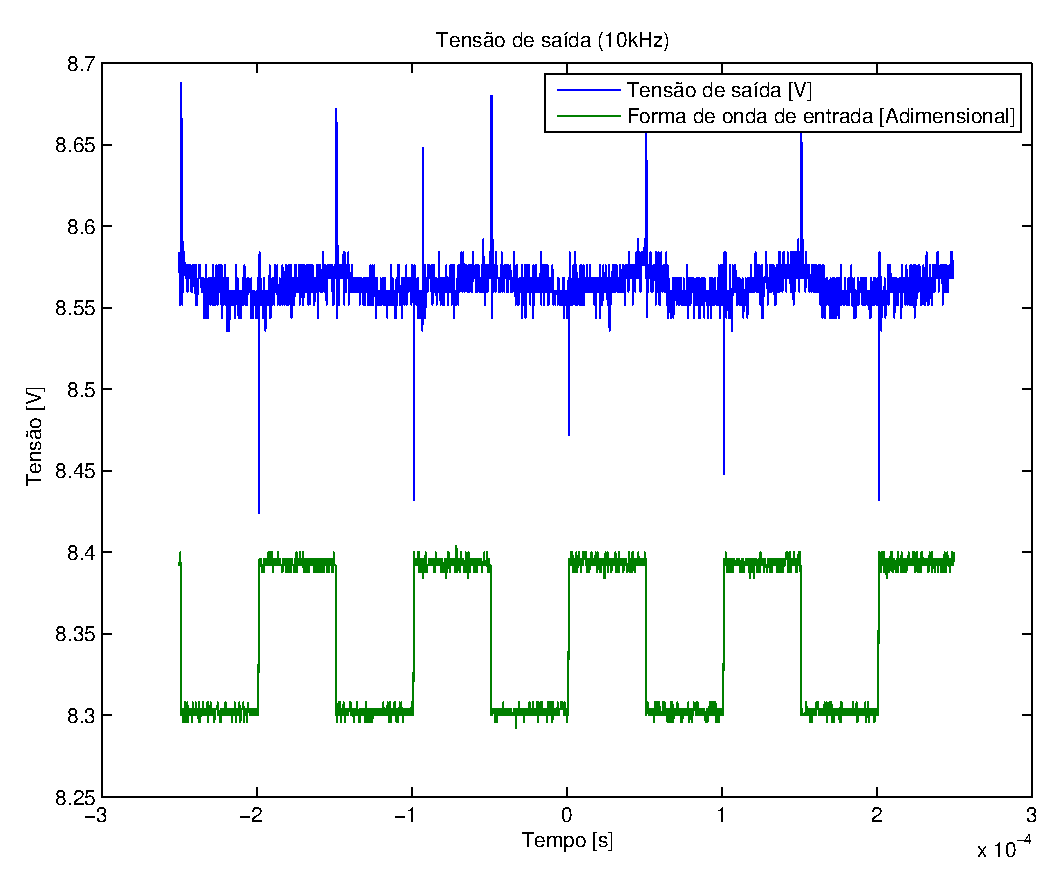
\includegraphics[width=\textwidth]{Dados/buck/t10k}
		\caption{10 kHz}
	\end{subfigure}
	\caption{Tensão de saída conversor buck em diferentes frequências de chaveamento ($D=50\%$)}
	\label{fig:but}
\end{figure}
\begin{figure}[H]
	\begin{subfigure}[b]{0.3\textwidth}
		\centering
		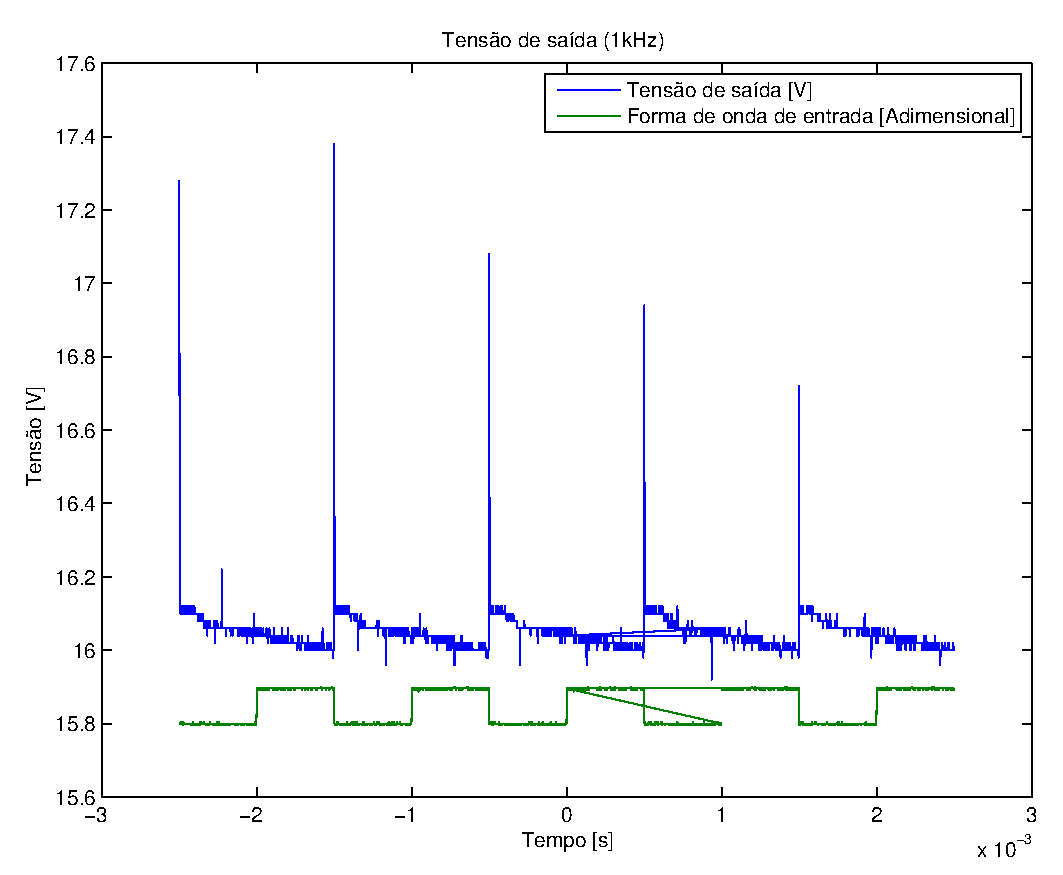
\includegraphics[width=\textwidth]{Dados/boost/t1k}
		\caption{1 kHz}
	\end{subfigure}
	\begin{subfigure}[b]{0.3\textwidth}
		\centering
		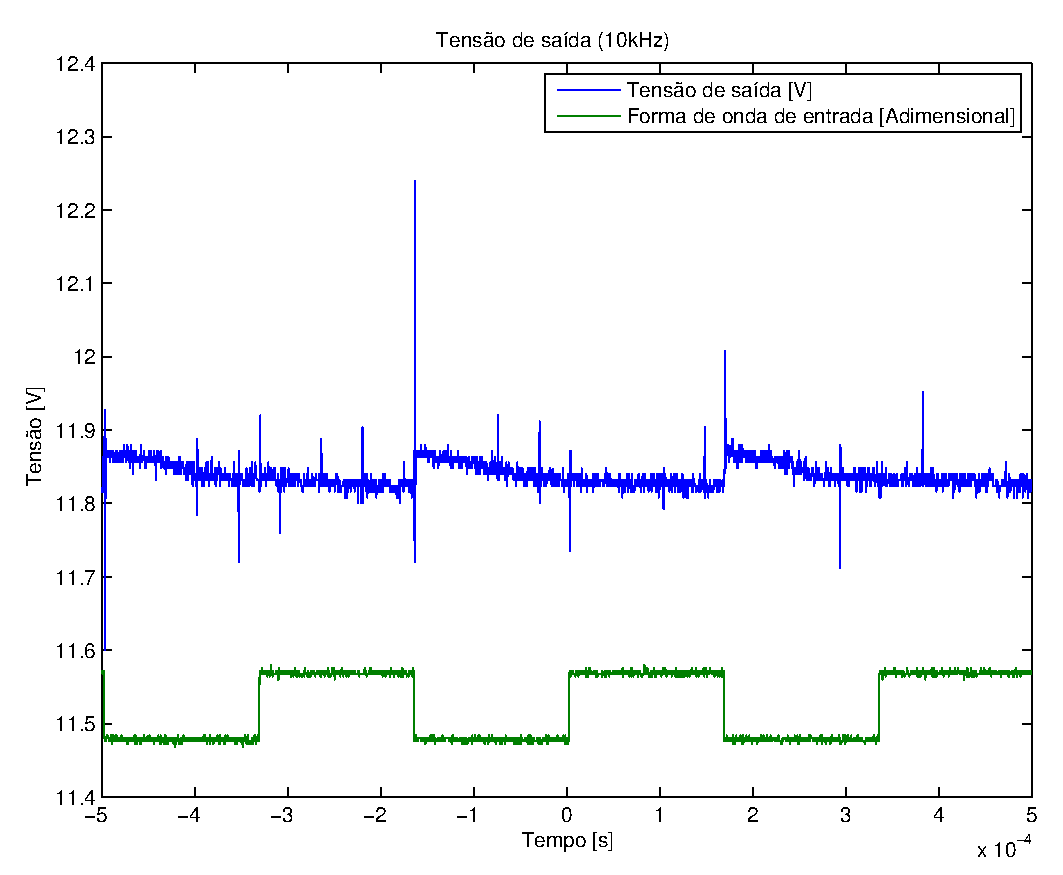
\includegraphics[width=\textwidth]{Dados/boost/t3k}
		\caption{3 kHz}
	\end{subfigure}
	\begin{subfigure}[b]{0.3\textwidth}
		\centering
		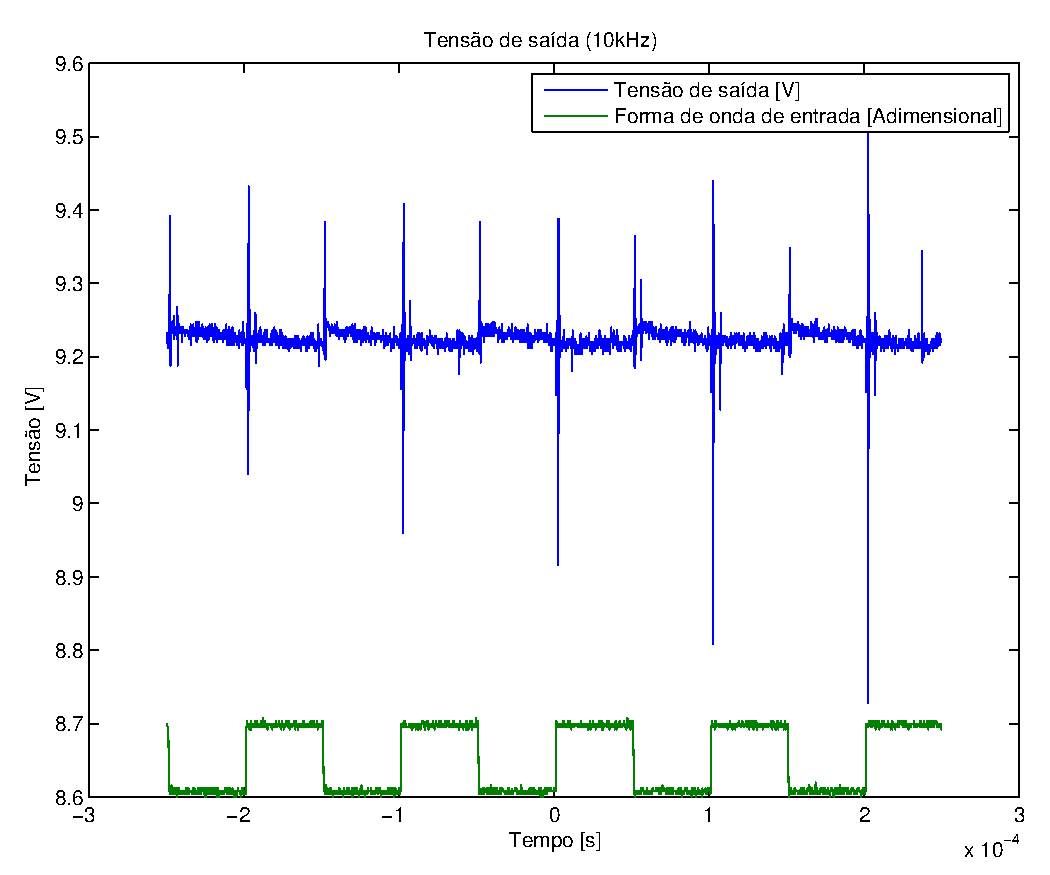
\includegraphics[width=\textwidth]{Dados/boost/t10k}
		\caption{10 kHz}
	\end{subfigure}
	\caption{Tensão de saída conversor boost em diferentes frequências de chaveamento ($D=50\%$)}
	\label{fig:bot}
\end{figure}

Para o cálculo da indutância limite $L_b$ para operação em condução contínua recorremos à equação a seguir, obtendo os resultados da tabela \ref{tab:Lb} para $D=50\%$, e $R=43\Omega$. Utilizamos os valores de frequência de chaveamento utilizados para adquirir os dados das figuras \ref{fig:but} e \ref{fig:bot}: $1kHz$, $3kHz$ e $10kHz$.

\begin{equation}
L_b = \frac{(1-D)R}{2f_s}	
\end{equation}

\begin{table}[H]
	\centering
	\caption{Indutância limite $L_b$ calculada para diferentes frequências de chaveamento}
	\label{tab:Lb}
	\begin{tabular}{|l|l|l|l|}
		\hline
		\multicolumn{1}{|c|}{\multirow{2}{*}{$f_s\ (kHz)$}} & 
		\multicolumn{2}{c|}{$v_R\ (V)$} & 
		\multicolumn{1}{c|}{\multirow{2}{*}{$L_b\ (H)$}} \\ \cline{2-3}
		\multicolumn{1}{|c|}{} 	& Buck           & Boost          & 
		\multicolumn{1}{c|}{}                          					  \\ \hline
		1     					& 11.4           & 16.1           & 10.75 \\ \hline
		3     					& 10.3           & 11.9           & 3.58  \\ \hline
		10    					& 8.56           & 9.23           & 1.07  \\ \hline
	\end{tabular}
\end{table}	

\section{Buck x Divisor de tensão}

Embora tenha maior complexidade, custo e volume, utilizando o conversor controlado Buck para fazer uma diminuição de tensão conseguimos diminuir as perdas por dissipação. Isto acontece pois o circuito que cuida da queda de tensão é composto, em sua maior parte, por dispositivo semicondutor, indutor e capacitor. Estes componentes possuem resistência equivalente menor do que a resistência necessária para um divisor de tensões. Desta maneira, tratando-se de eletrônica de potência, é viável a utilização de um conversor Buck.

\bibliography{mybib}
\end{document}

